En el estudio de la transmisión de señales (analógicas o digitales), es necesario diseñar el sistema para transmitir información que, a priori, no es conocida en detalle. Por ejemplo, la señal de voz de la radio AM/FM no se conoce hasta el momento de la transmisión. Lo mismo ocurre en la transmisión digital: típicamente podemos conocer \emph{estadísticamente} como se comportan los datos, pero no exactamente qué es lo que se va a transmitir. Debemos entonces poder diseñar y analizar los sistemas de transmisión para que respondan de manera adecuada a este conjunto posible de señales, de las cuales no conocemos exactamente más que sus propiedades estadísticas.

Es por ello esencial introducir el concepto de \emph{proceso estocástico} o aleatorio, que permite modelar este comportamiento. Comenzaremos en tiempo discreto para luego pasar a tiempo continuo, ya que ambos serán necesarios en el estudio de la modulación digital. Remitimos al apéndice \ref{app:probabilidad} para un resumen de los conceptos previos requeridos de probabilidad y variables aleatorias.

\section{Proceso estocástico de tiempo discreto}

Comencemos por definir el objeto de trabajo:
\begin{definicion}\label{def:proceso_td}
    Un \emph{proceso estocástico de tiempo discreto} es una sucesión de variables aleatorias $\{a_k:k\in\mathbb{Z}\}$ definidas en un espacio de probabilidad y que toman valores en un conjunto de símbolos $\{s_1,\ldots,s_M\}$ (espacio discreto) o valores en $\mathbb{R}$ (espacio continuo).
\end{definicion}

Observemos que la definición anterior no implica que los símbolos o muestras $a_k$ son independientes entre sí, es decir, pueden tener \emph{correlación} entre ellas. La distribución de un proceso estocástico depende precisamente de cuál es la probabilidad de observar cualquier secuencia de símbolos. En general esto es difícil de calcular por lo que definiremos algunas magnitudes de interés.

\begin{definicion}\label{def:media_var_td}
    Se definen la \emph{media} y \emph{varianza} del proceso como:
    \begin{equation*}
        \mu_k := \E{a_k}, \quad \sigma^2_k := \E{(a_k-\mu_k)^2} = \E{a_k^2} - \mu_k^2.
    \end{equation*}
    Por último definimos la \emph{potencia} del proceso como:
    \begin{equation*}
        P_k := \E{a_k^2} = \mu_k^2 + \sigma_k^2.
    \end{equation*}
\end{definicion}
Notar que en principio estas dependen de $k$, que es el índice de tiempo. Esto es, si la estadística del proceso cambia a lo largo del tiempo, también lo harán estas magnitudes.

Para capturar la dependencia del proceso introducimos la siguiente:
\begin{definicion}\label{def:autocorrelacion_noest_td}
    Se define la \emph{autocorrelación} de un proceso $\{a_k\}$ como:
    \begin{equation*}
        R(k_1,k_2) = \E{a_{k_1}a_{k_2}}
    \end{equation*}
\end{definicion}
Esta magnitud evalúa cuan ``alineados'' o ``similares'' son las muestras del proceso en los tiempos $k_1$ y $k_2$. En particular observemos que $R(k,k)=P_k$.

Sin embargo, todas estas magnitudes dependen del tiempo específico en que miremos. Es aquí que conviene introducir la noción de \emph{proceso estacionario}, que son aquellos procesos estocásticos cuyas propiedades estadísticas son invariantes en el tiempo, es decir la distribución de las observaciones $a_k$ o de las parejas $(a_{k_1},a_{k_2})$ no depende de $k$. En particular:
\begin{itemize}
    \item $\E{a_k} = \mu$, $\textrm{Var}(a_k)=\sigma^2$ y $P=\E{a_k^2}$ deben ser constantes.
    \item La autocorrelación satisface:
       \begin{equation*}
        R(k_1,k_2) = \E{a_{k_1}a_{k_2}} = \E{a_{0}a_{k_2-k_1}} = \E{a_{0}a_{l}} = R(0,l).
       \end{equation*}
       Es decir la autocorrelación solo depende de $l=k_2-k_1$, la distancia en el tiempo entre las observaciones o \emph{lag}.
\end{itemize}

A los efectos de trabajar con señales y modulación conviene entonces introducir la siguiente clase de procesos.
\begin{definicion}[Proceso WSS de tiempo discreto]
    Un proceso estocástico $\{a_k\}$ se dice \emph{estacionario en sentido amplio (WSS, wide-sense stationary)} si verifica:
    \begin{enumerate}
        \item $\E{a_k} = \mu$ constante.
        \item $R(a_{k_1},a_{k_2}) = R_a[k_2-k_1]$, siendo $R_a[l]$ una función únicamente del lag $l$, la distancia entre muestras.
    \end{enumerate}
\end{definicion}

\begin{ejemplo}[Variables aleatorias independientes]\label{ej:iid}
    Si las muestras $\{a_k\}$ son variables aleatorias independientes, de media $\mu$ y varianza $\sigma^2$ constantes, entonces se verifica la primera condición, y la autocorrelación además verifica:
    \begin{equation*}
        \E{a_k a_{k+l}} = \begin{cases}
        \E{a_k^2} = \mu^2 + \sigma^2 & \text{si }l=0, \\
        \E{a_k}\E{a_{k+\tau}} = \mu^2 & \text{si }l\neq 0.
        \end{cases}
    \end{equation*}
    Por lo tanto el proceso es WSS con $R_a[l] = \mu^2 + \sigma^2 \delta[l]$, siendo $\delta$ la delta de Dirac en tiempo discreto ($\delta[0]=1,\delta[l]=0, l\neq0$).

    \begin{center}
        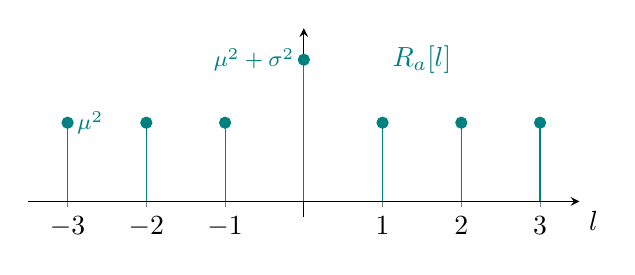
\begin{tikzpicture}
            \begin{axis}[ x=1cm, y=1cm, axis lines=middle,  
                    xlabel=$l$,
                    x label style={anchor=north west},
                    xmin=-3.5,xmax=3.5,ymin=-.2,ymax=2.2,
                    ytick=\empty,
                    clip=false,
                    ]
                \addplot+[teal,ycomb, mark options={teal}] plot coordinates {(-3,1) (-2,1) (-1,1) (0,1.8) (1,1) (2,1) (3,1)};
                \node[teal] at (axis cs:1.5,1.8) {$R_a[l]$};
                \node[teal,left] at (axis cs:0,1.8) {\footnotesize $\mu^2+\sigma^2$};
                \node[teal, right] at (axis cs:-3,1) {\footnotesize $\mu^2$};
            \end{axis}
        \end{tikzpicture}
    \end{center}
\end{ejemplo}

\begin{ejemplo}[Símbolos dependientes]\label{ej:markov source}
Consideremos una fuente que genera una secuencia de símbolos $\{a_k\}\in\{-1,1\}$ con la propiedad de que $\p{a_{k+1}=-1 \mid a_k=1} = \p{a_{k+1}=1 \mid a_k=-1} = \alpha$. Aquí $\alpha$ representa la probabilidad de ``cambiar de estado''. Si $\alpha\to 0$ la señal tiene rachas largas de $1$ y $-1$. Si $\alpha\to 1$ alterna periódicamente.

Es evidente que, en estado estacionario, por ser el sistema simétrico, $\p{a_k=1} = \p{a_k=-1} = 1/2$ por lo que en particular $\mu = \E{a_k} = 0$. La autocorrelación $R_a[l]$ puede calcularse por métodos que no veremos aquí y vale:
\begin{equation*}
    R_a[\tau] = (1-2\alpha)^{|l|}.
\end{equation*}

    \begin{center}
        \begin{tikzpicture}
            \begin{axis}[ x=1cm, y=1.2cm, axis lines=middle,  
                    xlabel=$l$,
                    x label style={anchor=north west},
                    xmin=-5.5,xmax=5.5,ymin=-.2,ymax=2,
                    ytick=\empty,
                    clip=false,
                    ]
                \addplot+[teal,ycomb, mark options={teal},samples = 11, domain=-5:5] {.5^abs(x)};
                \node[teal] at (axis cs:2.5,1.5) {$R_a[l], \; \alpha=1/4$};
            \end{axis}
        \end{tikzpicture}
    \end{center}

\end{ejemplo}

Listamos a continuación algunas propiedades de la autocorrelación:
\begin{enumerate}
    \item $R_a[l] = \E{a_k a_{k+l}} = \E{a_{k-l} a_k} = R_a[-l]$.
    \item $R_a[0] = \E{a_k^2} = P$.
    \item $|R_a[l]| = |\E{a_k a_{k+l}}| \leqslant \sqrt{\E{a_k^2}\E{a_{k+l}^2}} =\sqrt{P^2} = P = R_a[0]$. 
    
    Es decir, en módulo la autocorrelación es máxima en $0$. La desigualdad anterior surge de la desigualdad de Cauchy-Schwarz para variables aleatorias.
\end{enumerate}

La autocorrelación es la expresión temporal de cómo se repite (en promedio) la señal. Es por ello que a los efectos de analizar el filtrado y modulación de señales aleatorias interesa definir una expresión en el dominio de la frecuencia.

\begin{definicion}[Densidad espectral de potencia (tiempo discreto)]
    Se define la \emph{densidad espectral de potencia} de un proceso WSS de tiempo discreto con autocorrelación $R_a(\tau)$ como:
    \begin{equation}\label{def:dep_discreta}
        S_a(\phi) = \sum_{l=-\infty}^\infty R_a[l] e^{-j2\pi l \phi},
    \end{equation}
    es decir, la TFTD de la autocorrelación.
\end{definicion}

Esta función es periódica de período $1$ como función de $\phi$. La interpretación de $\phi$ es de \emph{frecuencia normalizada}, $f/f_s$ siendo $f_s$ la frecuencia de muestras de la señal. En general analizaremos el comportamiento de $S_a(\phi)$ para $\phi\in[-1/2,1/2]$ (correspondiente al intervalo $[-f_s/2,f_s/2]$ de frecuencias observables),

Al ser $S_a$ la TFTD de $R_a$, notemos que podemos recuperar la autocorrelación de la densidad espectral como:
\begin{equation*}
    R_a[l] = \int_{-\frac12}^{\frac12} S_a(\phi) e^{j2\pi l \phi} d\phi.
\end{equation*}

Algunas propiedades de la densidad espectral de potencia son:
\begin{enumerate}
    \item $S_a(\phi)$ es real y positiva.
    \item Para señales reales, $S_a(\phi)=S_a(-\phi)$ (función par).
    \item \begin{equation*}
    P = R_a[0] = \int_{-\frac12}^{\frac12} S_a(\phi) d\phi
    \end{equation*}
\end{enumerate}
Es decir, el área bajo la gráfica de $S_a$ (en un período) es igual a la potencia de la señal. En ese sentido, $S_a$ nos indica \emph{cómo se distribuye la potencia} a lo largo de las frecuencias observables.

\begin{ejemplo}
    Para el proceso independiente del Ejemplo \ref{ej:iid}, la densidad espectral de potencia queda:
    \begin{equation*}
        S_a(\phi) = \sum_{l=-\infty}^\infty \left[\mu^2 + \sigma^2 \delta(k)\right]e^{-j2\pi\phi\tau} = \sigma^2 + \mu^2 \sum_{l=-\infty}^\infty e^{-j2\pi\phi\tau} = \sigma^2 + \mu^2 \sum_{l=-\infty}^\infty \delta(\phi-l),
    \end{equation*}
donde en el último paso usamos la suma de Poisson.
    \begin{center}
    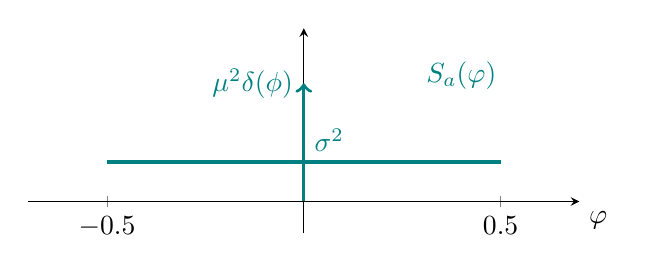
\begin{tikzpicture}
        \begin{axis}[ x=5cm, y=2cm, axis lines=middle,  
                xlabel=$\varphi$,
                x label style={anchor=north west},
                xmin=-.7,xmax=.7,ymin=-.2,ymax=1.1,
                ytick=\empty,
                xtick = {-.5,.5},
                clip=false,
                ]
            \addplot[teal, samples = 100, domain=-.5:.5, very thick] {1/4} node[midway,above right] {$\sigma^2$};
            \node[teal] at (axis cs:.4,.8) {$S_a(\varphi)$};
            \draw[teal,very thick, ->] (axis cs:0,0) -- (axis cs:0,.75) node[left] {$\mu^2 \delta(\phi)$};
        \end{axis}
    \end{tikzpicture}
\end{center}

\end{ejemplo}

\begin{ejemplo}
    Para la señal aleatoria con símbolos dependientes del Ejemplo \ref{ej:markov source}, la densidad espectral de potencia queda:
    \begin{align*}
        S_a(\phi) &= \sum_{\tau = -\infty}^\infty (1-2\alpha)^{|\tau|} e^{-j2\pi\phi \tau} = 1 + \sum_{l=1}^\infty \left[(1-2\alpha)e^{-j2\pi\phi }\right]^l + \sum_{l=1}^\infty \left[(1-2\alpha)e^{j2\pi\phi}\right]^l \\
        &= 1 + \frac{(1-2\alpha)e^{-j2\pi\phi}}{1-(1-2\alpha)e^{-j2\pi\phi}} + \frac{(1-2\alpha)e^{j2\pi\phi}}{1-(1-2\alpha)e^{j2\pi\phi}}\\
        &= \frac{2\alpha(1-\alpha)}{1-2\alpha(1-\alpha) - (1-2\alpha)\cos(2\pi\phi)}.
    \end{align*}

    Por ejemplo, para $\alpha=1/4$ queda:
    \begin{center}
        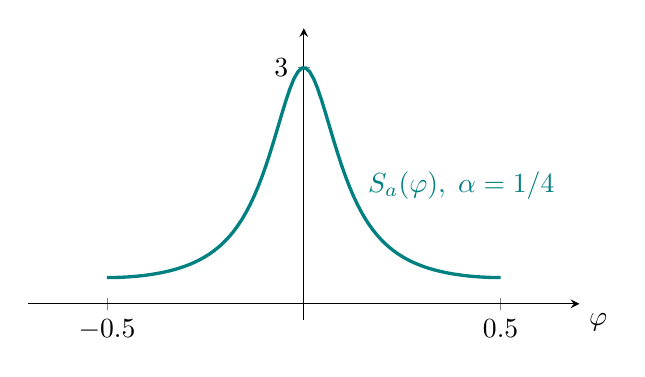
\begin{tikzpicture}
            \begin{axis}[ x=5cm, y=1cm, axis lines=middle,  
                    xlabel=$\varphi$,
                    x label style={anchor=north west},
                    xmin=-.7,xmax=.7,ymin=-.2,ymax=3.5,
                    ytick={3},
                    xtick = {-.5,.5},
                    clip=false,
                    ]
                \addplot[teal, samples = 100, domain=-.5:.5, very thick] {(3/8)/(1-(3/8)-(1/2)*cos(deg(2*pi*x)))};
                \node[teal] at (axis cs:.4,1.5) {$S_a(\varphi), \; \alpha=1/4$};
            \end{axis}
        \end{tikzpicture}
    \end{center}
\end{ejemplo}

Por último, introducimos una última noción:
\begin{definicion}
    Un proceso es \emph{ergódico} si una realización cualquiera es representativa de la estadística del proceso.
\end{definicion}

La anterior es una definición informal, pero la idea general es que si promediamos los valores de una traza del proceso, entonces recuperamos los valores medios. En particular:
\begin{align*}
    \left\langle a \right\rangle  &= \lim_{N\to\infty} \frac{1}{2N+1}\sum_{k=-N}^N a_k = E[a_k] = \mu, \\
    \left\langle a^2 \right\rangle &= \lim_{N\to\infty} \frac{1}{2N+1}\sum_{k=-N}^N a_k^2 = E[a_k^2] = P, \\
    \left\langle a_k a_{k+l}\right\rangle &= \lim_{N\to\infty} \frac{1}{2N+1}\sum_{k=-N}^N a_k a_{k+l} = E[a_k a_{k+l}] = R_a[l].
\end{align*}
Es decir, los valores medios de una señal dada suficientemente larga aproximan la esperanza, similar a lo que ocurre en la ley de grandes números. En particular se requiere estacionariedad (porque el límite no depende de $k$). En este curso asumiremos siempre que los procesos con que trabajamos son WSS y ergódicos.

\section{Proceso estocástico de tiempo continuo}

Generalizamos ahora las definiciones ya vistas al caso de tiempo continuo, lo que nos servirá por ejemplo para modelar señales analógicas que son moduladas por una señal digital, o también el ruido que afecta a un sistema.

\begin{definicion}\label{def:proceso_tc}
    Un \emph{proceso estocástico de tiempo continuo} es una función aleatoria $x(t,\omega)$ a valores reales, con $\omega$ sorteada en un espacio de probabilidad.
\end{definicion}

La principal diferencia es que ahora el sorteo en el espacio determina toda una función $x(t)$ para cada posible realización del experimento (valor de $\omega$). En la FIgura \ref{fig:realizaciones} se muestra un ejemplo de esto. En general, denotaremos por $x(t)$ a la señal o proceso aleatorio, sin indicar la dependencia con el espacio de probabilidad subyacente.

\begin{figure}
    \begin{center}
        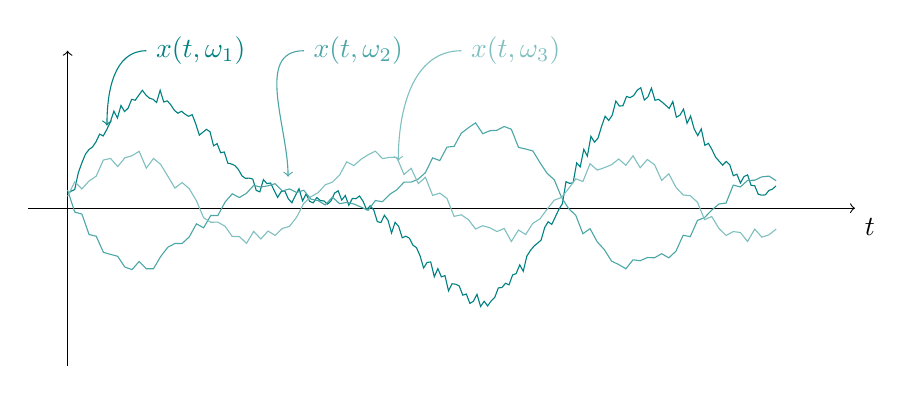
\begin{tikzpicture}
            \draw [->] (-0.5,0) -- (10,0) node[below right] {$t$};
            \draw [->] (0,-2) -- (0,2);
            \draw [samples=200,domain=0:9, teal] plot (\x,{0.15+sin(\x r)*(1+cos(\x r +1))+0.1*rand});
            \draw [->, teal] (1,2) node [anchor=west] {$x(t,\omega_1)$} to [out=180,in = 90] (0.5,1.05);
            \draw [samples=100,domain=0:9,color=teal!70!white] plot (\x, {0.15-sin(\x r)*(0.5+cos(\x r +1))+0.1*rand});
            \draw [->,color=teal!70!white] (3,2) node [anchor=west] {$x(t,\omega_2)$} to [out=180,in=90] (2.8,0.4);
            \draw [samples=100,domain=0:9,color=teal!50!white] plot (\x, {0.15+sin(\x r)*(cos(\x r +1))+0.1*rand});
            \draw [->,color=teal!50!white] (5,2) node [anchor=west] {$x(t,\omega_3)$} to [out=180,in=90] (4.2,0.6);
        \end{tikzpicture}
        \caption{Diferentes realizaciones de un proceso estocástico de tiempo continuo}\label{fig:realizaciones}
    \end{center}
\end{figure}

Dado un proceso estocástico $x(t)$, podemos definir:
\begin{definicion}\label{def:media_var_tc}
    Se definen la función \emph{media} y \emph{varianza} del proceso como:
    \begin{equation*}
        \mu(t) := \E{x(t)}, \quad \sigma^2(t) := \E{(x(t)-\mu(t))^2} = \E{x(t)^2} - \mu(t)^2.
    \end{equation*}
    Por último definimos la \emph{potencia} del proceso como:
    \begin{equation*}
        P(t) := \E{x(t)^2} = \mu(t)^2 + \sigma(t)^2.
    \end{equation*}
\end{definicion}

Tenemos a su vez el análogo a la autocorrelación de tiempo discreto.
\begin{definicion}\label{def:autocorrelacion_noest_tc}
    Se define la \emph{autocorrelación} de un proceso estocástico de tiempo continuo $x(t)$ como la función de dos variables:
    \begin{equation*}
        R(s,t) = \E{x(s)x(t)}.
    \end{equation*}
\end{definicion}
Observemos  que $R(t,t)=P(t)$.

Nuevamente, todas las magnitudes anteriores dependen en principio de los momentos del tiempo en que miramos el proceso. Buscamos entonces trabajar con procesos \emph{estacionarios} cuya estadística no cambie con el tiempo.
\begin{definicion}[Proceso WSS de tiempo continuo]
    Un proceso estocástico $x(t)$ se dice \emph{estacionario en sentido amplio (WSS, wide-sense stationary)} si verifica:
    \begin{enumerate}
        \item $\E{x(t)} = \mu$ constante.
        \item $R(s,t) = \E{x(s)x(t)} = \E{x(0)x(t-s)} =  R_x(\tau)$, siendo $R_x(\tau)$ una función únicamente de $\tau = t-s$, el tiempo entre muestras.
    \end{enumerate}
\end{definicion}

Tenemos además los análogos de tiempo continuo de la función de autocorrelación.\begin{enumerate}
    \item $R_x(\tau) = \E{x(t) x(t-\tau)} = \E{x(t+\tau)x(t)} = R_x(-\tau)$, es decir $R_x$ es una función par.
    \item $R_x(0) = \E{x(t)^2} = P$.
    \item $|R_x(\tau)| = |\E{x(t)x(t-\tau)}| \leqslant \sqrt{\E{x(t)^2}\E{x(t-\tau)}^2} =\sqrt{P^2} = P = R_a(0)$. 
Nuevamente, el módulo de la autocorrelación es máximo en $0$. La desigualdad anterior surge de la desigualdad de Cauchy-Schwarz para variables aleatorias.
\end{enumerate}

Por último, un proceso es además ergódico si cada trayectoria $x(t)$ es representativa de la estadística del proceso, como antes. En particular:
\begin{align*}
    \left\langle x \right\rangle  &= \lim_{T\to\infty} \frac{1}{2T}\int_{-T}^T x(t)dt = \E{x(t)} = \mu, \\
    \left\langle (x-\mu)^2 \right\rangle  &= \lim_{T\to\infty} \frac{1}{2T}\int_{-T}^T (x(t)-\mu)^2 dt = \E{(x(t)-\mu)^2} = \sigma^2, \\
    \left\langle x^2 \right\rangle &= \lim_{T\to\infty} \frac{1}{2T}\int_{-T}^T x(t)^2 dt = \E{x(t)^2} = P, \\
    \left\langle x(t) x(t-\tau) \right\rangle &= \lim_{T\to\infty} \frac{1}{2T}\int_{-T}^T x(t)x(t-\tau)dt = E[x(t)x(t-\tau)] = R_x(\tau).
\end{align*}
Es decir, los valores medios de una señal dada suficientemente larga aproximan la esperanza, similar a lo que ocurre en la ley de grandes números. Esto requiere estacionariedad (porque el límite no depende de $t$). En este curso asumiremos siempre que los procesos con que trabajamos son WSS y ergódicos. En particular, $\mu^2$ representa la potencia de continua de la señal, $\sigma^2$ la potencia de ``alterna'' y $P$ la potencia total.

A continuación algunos ejemplos de procesos estacionarios de tiempo continuo.

\begin{ejemplo}[Sinusoide de fase aleatoria]\label{ej:cos random phase}
Consideremos el siguiente proceso aleatorio:
\begin{equation*}
    x(t) = A\cos(2\pi f_0 t + \theta)
\end{equation*}
con $\theta$ aleatorio y distribuido uniformemente en el intervalo $[0,2\pi]$. Este proceso modela el fenómeno de observar una señal sinusoidal de frecuencia fija $f_0$, pero sin referencia a su tiempo de origen, es decir, no conocemos la fase del oscilador que la genera. Calculemos:
\begin{align*}
    \E{x(t)} &= \E{A\cos(2\pi f_0 t + \theta)} = \int_0^{2\pi} A\cos(2\pi f_0 t + \theta) \frac{1}{2\pi} d\theta \\
    &= \frac{A}{2\pi}\int_0^{2\pi} A\cos(2\pi f_0 t + \theta)  d\theta = 0.
\end{align*}
Notar que estamos integrando en $\theta$, por lo que la integral es en un período de la función $\cos$. Entonces $E[x(t)] = \mu = 0$ constante. Calculemos la autocorrelación:
\begin{align*}
    \E{x(s)x(t)} &= \E{A\cos(2\pi f_0 s + \theta)A\cos(2\pi f_0 t + \theta)} = A^2 \int_0^{2\pi} \cos(2\pi f_0 s + \theta) \cos(2\pi f_0 t + \theta) \frac{1}{2\pi} d\theta \\
    &= \frac{A^2}{2}\int_0^{2\pi} \left[\cos(2\pi f_0 (t-s)) + \cos(2\pi f_0 (t+s) + 2\theta)\right] \frac{1}{2\pi} d\theta \\
    &= \frac{A^2}{2} \left[\cos(2\pi f_0 (t-s)) \overbrace{\int_0^{2\pi} \frac{1}{2\pi}d\theta}^{=1} + \overbrace{\int_0^{2\pi} \cos(2\pi f_0 (t+s) + 2\theta) \frac{1}{2\pi} d\theta}^{=0}\right] \\
    &= \frac{A^2}{2}\cos(2\pi f_0 (t-s)) = R_x(\tau).
\end{align*}
Por lo tanto el proceso es WSS, ya que la media es constante y la autocorrelación $R_x$ solo depende de la distancia entre muestras. La potencia del proceso $R_x(0) = A^2/2$, que corresponde al valor RMS de una sinusoide de amplitud $A$.
\end{ejemplo}

Algunas observaciones importantes sobre el ejemplo anterior: en primer lugar, la autocorrelación es periódica de período $T_0 = 1/f_0$, la frecuencia base. Esto es porque la señal se repite exactamente igual cada tiempo $T_0$ (de hecho, la autocorrelación vuelve a ser máxima en $f=kf_0$). En segundo lugar, notar que la autocorrelación no lleva información de fase. Por ejemplo, si el Ejemplo \ref{ej:cos random phase} cambiamos $\cos$ por $\sin$, la autocorrelación \emph{no cambia}.\footnote{Notar que $\sin(\tau)$ no puede ser una función de autocorrelación adecuada, ya que vale $0$ en $\tau=0$ y es impar.} 

\begin{ejemplo}[Onda binaria aleatoria]\label{ej:onda binaria aleatoria}

    En este ejemplo, consideramos una señal aleatoria de tipo onda cuadrada, pero cuyas amplitudes están controladas por símbolos binarios $a_k=\pm 1$ equiprobables. Este es nuestro primer ejemplo de modulación digital.
    
    Más concretamente, consideremos el proceso estocástico:
    \begin{equation*}
        x(t) = \sum_{k=-\infty}^\infty a_k p(t-kT_s + D),
    \end{equation*}
    siendo:
    \begin{itemize}
        \item $a_k$ una secuencia de símbolos independientes con $\p{a_k=1}=\p{a_k=-1}$.
        \item $p(t)$ el pulso de alto $1$ y duración $T_s$, el tiempo de símbolo.
        \item $D$ una v.a. independiente de las anteriores, y con distribución Uniforme en $[0,T_s]$.
    \end{itemize}
    Nuevamente aquí $D$ juega el rol de una ``fase aleatoria'', en el sentido de que no sabemos cuándo la señal comenzó a transmitir y la observamos en un momento aleatorio del tiempo, como se ve en la Figura \ref{fig:onda binaria aleatoria}. Sin este paso, el proceso no sería estacionario, ya que los momentos de cambio de símbolo $kT_s$ serían ``especiales''.

    \begin{figure}
        \begin{center}
            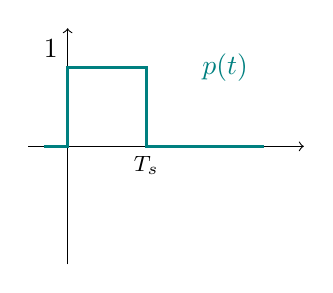
\begin{tikzpicture}
                \draw [->] (-0.5,0) -- (3,0);
                \draw [->] (0,-1.5) -- (0,1.5);                               \node at (0,1) [anchor=south east] {$1$}; 
                \draw[very thick, teal] (-.3,0) -- (0,0) -- (0,1) -- (1,1) -- (1,0) -- (2.5,0);
                \node at (1,0) [below] {\footnotesize $T_s$}; 
                \node at (2,1) [teal,] {$p(t)$}; 
            \end{tikzpicture} \hspace{1cm}
            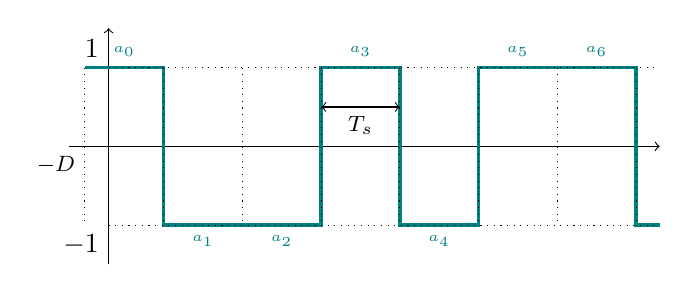
\begin{tikzpicture}
                \draw [->] (-0.5,0) -- (7,0);
                \draw [->] (0,-1.5) -- (0,1.5);
                \node at (0,1) [anchor=south east] {$1$}; 
                \node at (0,-1) [anchor=north east] {$-1$};
                \node at (-.3,0) [anchor=north east] {\footnotesize $-D$};
                \draw[very thick, teal] (-.3,1) --node[midway,above] {\tiny $a_0$} (.7,1) -- (.7,-1) --node[midway,below] {\tiny $a_1$} (1.7,-1) --node[midway,below] {\tiny $a_2$} (2.7,-1)-- (2.7,1) --node[midway,above] {\tiny $a_3$} (3.7,1) -- (3.7,-1) --node[midway,below] {\tiny $a_4$} (4.7,-1) -- (4.7,1) --node[midway,above] {\tiny $a_5$} (5.7,1) --node[midway,above] {\tiny $a_6$} (6.7,1) -- (6.7,-1) -- (7,-1);
                \draw [dotted,thin] (0,1) -- (7,1);
                \draw [dotted,thin] (0,-1) -- (7,-1);
                \foreach \x in {0,1,2,3,4,5,6,7} {
                  \draw [dotted,thin] (\x-.3,1) -- (\x-.3,-1);
                }

                \draw[<->] (2.7,.5) --node[midway,below] {\footnotesize $T_s$} (3.7,.5);
            \end{tikzpicture}
        \end{center}
        \caption{Pulso base y realización de una onda binaria aleatoria del Ejemplo \ref{ej:onda binaria aleatoria}.}\label{fig:onda binaria aleatoria}
    \end{figure}

    Calculemos media y autocorrelación de este proceso. Comenzamos por la media: para ello condicionamos a un valor de $D=z$ y luego integramos entre todos los posibles valores de esta variable uniforme, quedando:
    \begin{equation*}
        \E{x(t)} = \int_0^{T_s} \E{x(t)\mid D=z} \frac{1}{T_s} dz.
    \end{equation*}
    Ahora, dado $D=z$, observemos que:
    \begin{equation*}
        p(t-kT_s + z) = 1 \iff 0\leqslant t-kT_s +z < T_s \iff k\leqslant \frac{t + z}{T_s} < k+1.
    \end{equation*}
    Es decir, existe un único $k=k_0 = \left\lfloor \frac{t+z}{T_s}\right\rfloor$ tal que $p(t-k_0T_s + z) = 1$. Básicamente esto ocurre porque los pulsos no se solapan y por lo tanto en cada momento del tiempo $t$ observamos un único símbolo $a_k$. Entonces:
    \begin{equation*}
        \E{x(t)\mid D =  z} = P(a_{k_0} = 1) (1) + P(a_{k_0} = -1) (-1) = \frac{1}{2}-\frac{1}{2} = 0, 
    \end{equation*}
    de donde $\mu = \E{x(t)} = 0$ para todo $t$, es decir la señal tiene media constante y no tiene componente de continua.

    Pasemos ahora a calcular la correlación $R(t_1,t_2) = \E{x(t_1)x(t_2)}$.    Distinguimos dos casos:
    \begin{enumerate}
        \item Si $|t_1-t_2|>T_s$, entonces los símbolos observados en $t_1$ y $t_2$ son independientes, ya que pertenecen a pulsos distintos. Es decir, existen $k_1\neq k_2$ como antes, tales que $p(t_1-k_1T_s+z) = 1$ y $p(t_2-k_2T_s+z) = 1$. En ese caso:
        \begin{equation*}
          \E{x(t_1)x(t_2)\mid D=z} = \E{a_{k_1}a_{k_2}} = \E{a_{k_1}}\E{a_{k_2}} = 0,  
        \end{equation*}
        es decir no hay correlación para $|t_2-t_1|\geqslant T_s$, a distancia más de un tiempo de símbolo.

        \item Si en cambio $|t_2-t_1|<T_s$, entonces los símbolos pueden corresponder al mismo pulso, o a pulsos consecutivos, dependiendo de la fase. Supongamos primero que $t_2>t_1$ y que $x(t_1)=a_k$. La observación crucial es que el tiempo de cambio de símbolo $T_{k+1}$ tiene distribución uniforme en $[t_1,t_1+T_s]$, por lo que:
        \begin{equation*}
            \begin{cases}
            x(t_1) = x(t_2) = a_k \quad  \text{Si } t_2-t_1 < T_{k+1}, \\
            x(t_1) = a_k, x(t_2) = a_{k+1} \quad  \text{Si } t_2-t_1 \geqslant T_{k+1}.
            \end{cases}
        \end{equation*}
        Por lo tanto:
        \begin{align*}
            \E{x(t_1)x(t_2)} &= \overbrace{\E{a_k^2}}^{=1} \p{T_{k+1}>t_2-t_1} + \overbrace{\E{a_ka_{k+1}}}^{=0}\p{T_{k+1}\leqslant t_2-t_1} \\
            &= 1-\frac{(t_2-t_1)}{T_s}. 
        \end{align*}
    \end{enumerate}

    Un razonamiento análogo para $t_2<t_1$ permite concluir que el proceso es WSS (la autocorrelación solo depende de $\tau=t_2-t_1$) y su función de autocorrelación es:
    \begin{equation}\label{eq:autocorrelacion onda binaria centrada}
        R_x(\tau) = 1-\frac{|\tau|}{T_s} \quad -T_s\leqslant \tau \leqslant T_s,
    \end{equation}
    y $0$ en otro caso.

    \begin{center}
        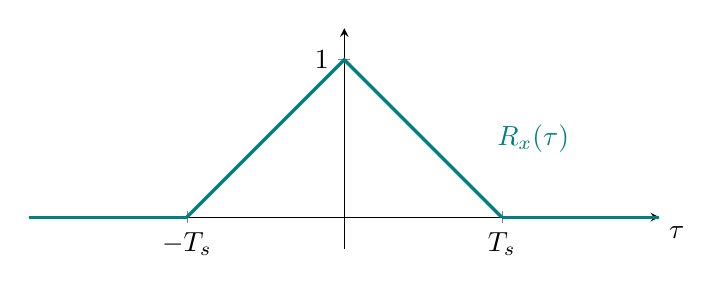
\begin{tikzpicture}
            \begin{axis}[ x=2cm, y=2cm, axis lines=middle,  
                        xlabel=$\tau$,
                        x label style={anchor=north west},
                        xmin=-2,xmax=2,ymin=-.2,ymax=1.2,
                        ytick={1},
                        xtick = {-1,1},
                        xticklabels = {$-T_s$,$T_s$},
                        clip=false,
                        ]
            \addplot [domain=-1:1, teal, very thick, samples=11] {1-abs(x)}; 
            \addplot [domain=-2:-1, teal, very thick, samples=2] {0}; 
            \addplot [domain=1:2, teal, very thick, samples=2] {0}; 
            \node[teal] at (axis cs: 1.2,.5) {$R_x(\tau)$};
            \end{axis}
        \end{tikzpicture}
    \end{center}
\end{ejemplo}





\begin{definicion}[Proceso Gaussiano]
    
\end{definicion}

\begin{definicion}[Ruido blanco Gaussiano (WGN)]
    
\end{definicion}